
\ifintegriereaufgaben

\section*{Orthogonalprojektion in \texorpdfstring{$\mathbb R^n$}{Rn} Aufgaben}\label{MA2-orthogonalprojektion-aufgaben}
Regeln und Beispiele, die zur Bearbeitung der Aufgaben hilfreich sind, finden Sie im Skript\wennreferenzvorhanden{MA2-orthogonalprojektion}{ (Abschnitt \abschnittsverweis{MA2-orthogonalprojektion})} und, falls Sie nicht weiterkommen, schauen Sie \hyperref[MA2-orthogonalprojektion-loesungen]{hier}.
\else
\section{Orthogonalprojektion in \texorpdfstring{$\mathbb R^n$}{Rn} Aufgaben}\label{MA2-orthogonalprojektion-aufgaben}

Regeln und Beispiele zu diesen Aufgaben finden Sie im Skript. Die L�sungen finden Sie \hyperref[MA2-orthogonalprojektion-loesungen]{hier}.
\fi

\begin{exercisebox}[�berbestimmtes Gleichungssystem]
	Gegeben ist das Gleichungssystem \[ A =
		 \left( \begin{array}{cc}
			2 & 1   \\
			6 & 2   \\
			-1 & 0
\end{array}\right) \,\left( \begin{array}{c}x_1 \\x_2\end{array}\right) = \left( \begin{array}{c} 1 \\5\\ c \end{array}\right)\,, \] wobei \(c\in\mathbb R\) eine beliebige reelle Zahl ist.

	\begin{itemize}
		\item[(a)] Bestimmen Sie eine L�sung des Gleichungssystems \(A\,\boldsymbol x = \boldsymbol b\). Hinweis: Schr�nken Sie, wenn n�tig, den der Wertebereich f�r die Konstante \(c\) ein.
		\item[(b)] Bestimmen Sie eine L�sung \(\boldsymbol x_*\) der Normalengleichung \(A^\intercal \, A \, \boldsymbol x = A^\intercal \,\boldsymbol b \).
		\item[(c)] Berechnen Sie das Residuum \(\boldsymbol r = A\, \boldsymbol x_* - \boldsymbol b\) und bestimmen Sie \(c\) so, dass \(\| \boldsymbol r\| = 0\) gilt und vergleichen Sie die resultierende L�sung \(\boldsymbol x_*\) mit der L�sung, die Sie unter (a) berechnet haben.
	\end{itemize}
\end{exercisebox}

\begin{exercisebox}[�berbestimmtes Gleichungssystem]
	Gegeben ist die lineare Abbildung \[ \mathcal A: \mathbb R^3 \to \mathbb R^4, \left( \begin{array}{c} x_1 \\x_2 \\ x_3\end{array}\right) \mapsto \left( \begin{array}{c} x_1 - x_2 + x_3 \\ 3\,x_1 + 2\,x_2 + x_3 \\ x_1 + 2\, x_2 + 4\, x_3 \\ -x_1 + 7\,x_2 + x_3 \end{array}\right) \]
	\begin{itemize}
		\item[(a)] Bestimmen Sie die Matrix \(A\), die die lineare Abbildung \(\mathcal A\) erzeugt\footnote{Gesucht ist also die Matrix \(A\), f�r die gilt \( \mathcal A: \boldsymbol x \mapsto A\,\boldsymbol x\), wobei \(A\,\boldsymbol x\) die Matrix-Vektor-Multiplikation ist.}
		\item[(b)] Der Bildbereich der Abbildung \(\mathcal A\) wird das Bild von \(A\) genannt und mit \(\mathrm{im}(A)\) notiert. Bestimmen Sie explizit eine Basis von \(\mathrm{im}(A)\).
		\item[(c)] Analysieren Sie die L�sbarkeit des Gleichungssystems \(A\,\boldsymbol x = \boldsymbol b\) f�r \(\boldsymbol b = (0, 2, 0, 2)^\intercal\).
		\item[(d)] Bestimmen Sie die L�sung der Normalengleichung und zeigen Sie rechnerisch, dass das Residuum senkrecht auf \(\mathrm{im}(A)\) steht.
		\item[(e)] Nennen Sie eine rechte Seite \(\boldsymbol b\), f�r die das lineare Gleichungssystem \(A\,\boldsymbol x = \boldsymbol b\) eindeutig l�sbar ist und �berpr�fen Sie rechnerisch, ob die L�sung auch die Normalengleichung l�st.
	\end{itemize}
\end{exercisebox}

\begin{exercisebox}[Koeffizienten Lineare Regression]
	F�r \(n\) Messerte \( \left( \tilde x_i,\, \tilde y_i\right) \) ist die Gerade \(g: x\mapsto a_1\cdot x + a_0\) mit den Koeffizienten
	\begin{equation}\label{koeffizienten_ausgleichsgerade} \left\{  \begin{array}{rcl}
				a_1 &=& \dfrac{ \sum\limits_{i=1}^n \left( x_i - \overline x\right) \cdot \left( y_i - \overline y\right)}{ \sum\limits_{i=1}^n \left( x_i - \overline x\right) \cdot \left( x_i - \overline x\right)}\,, \\[2ex]
				a_0 &=& \overline y - a_1 \, \overline x\,.
\end{array} \right.\end{equation}
	genau die Gerade, die die Summe aller Abstandsquadrate zwischen Funktions- und Messerten minimiert, f�r die also gilt \[ \sum\limits_{i=1}^n | g(x_i)-y_i|^2 = \mathrm{min}.\]

	\noindent \textbf{Hinweise:}
	\begin{itemize}
		\item Zeigen Sie die G�ltigkeit von \eqref{koeffizienten_ausgleichsgerade} mit Mitteln der Differentialrechnung.
		\item Mit \(\overline x\) bzw \(\overline y\) werden die arithmetischen Mittelwerte bezeichnet:
			\[ \begin{array}{rcl} \overline x &=& \dfrac1n\, \sum\limits_{i=1}^n x_i\,, \\ \overline y &=& \dfrac1n\, \sum\limits_{i=1}^n y_i\,. \end{array}\]
	\end{itemize}
\end{exercisebox}

%\begin{exercisebox}[L�sung der Normalengleichung]
%\begin{minipage}{0.35\textwidth}
%	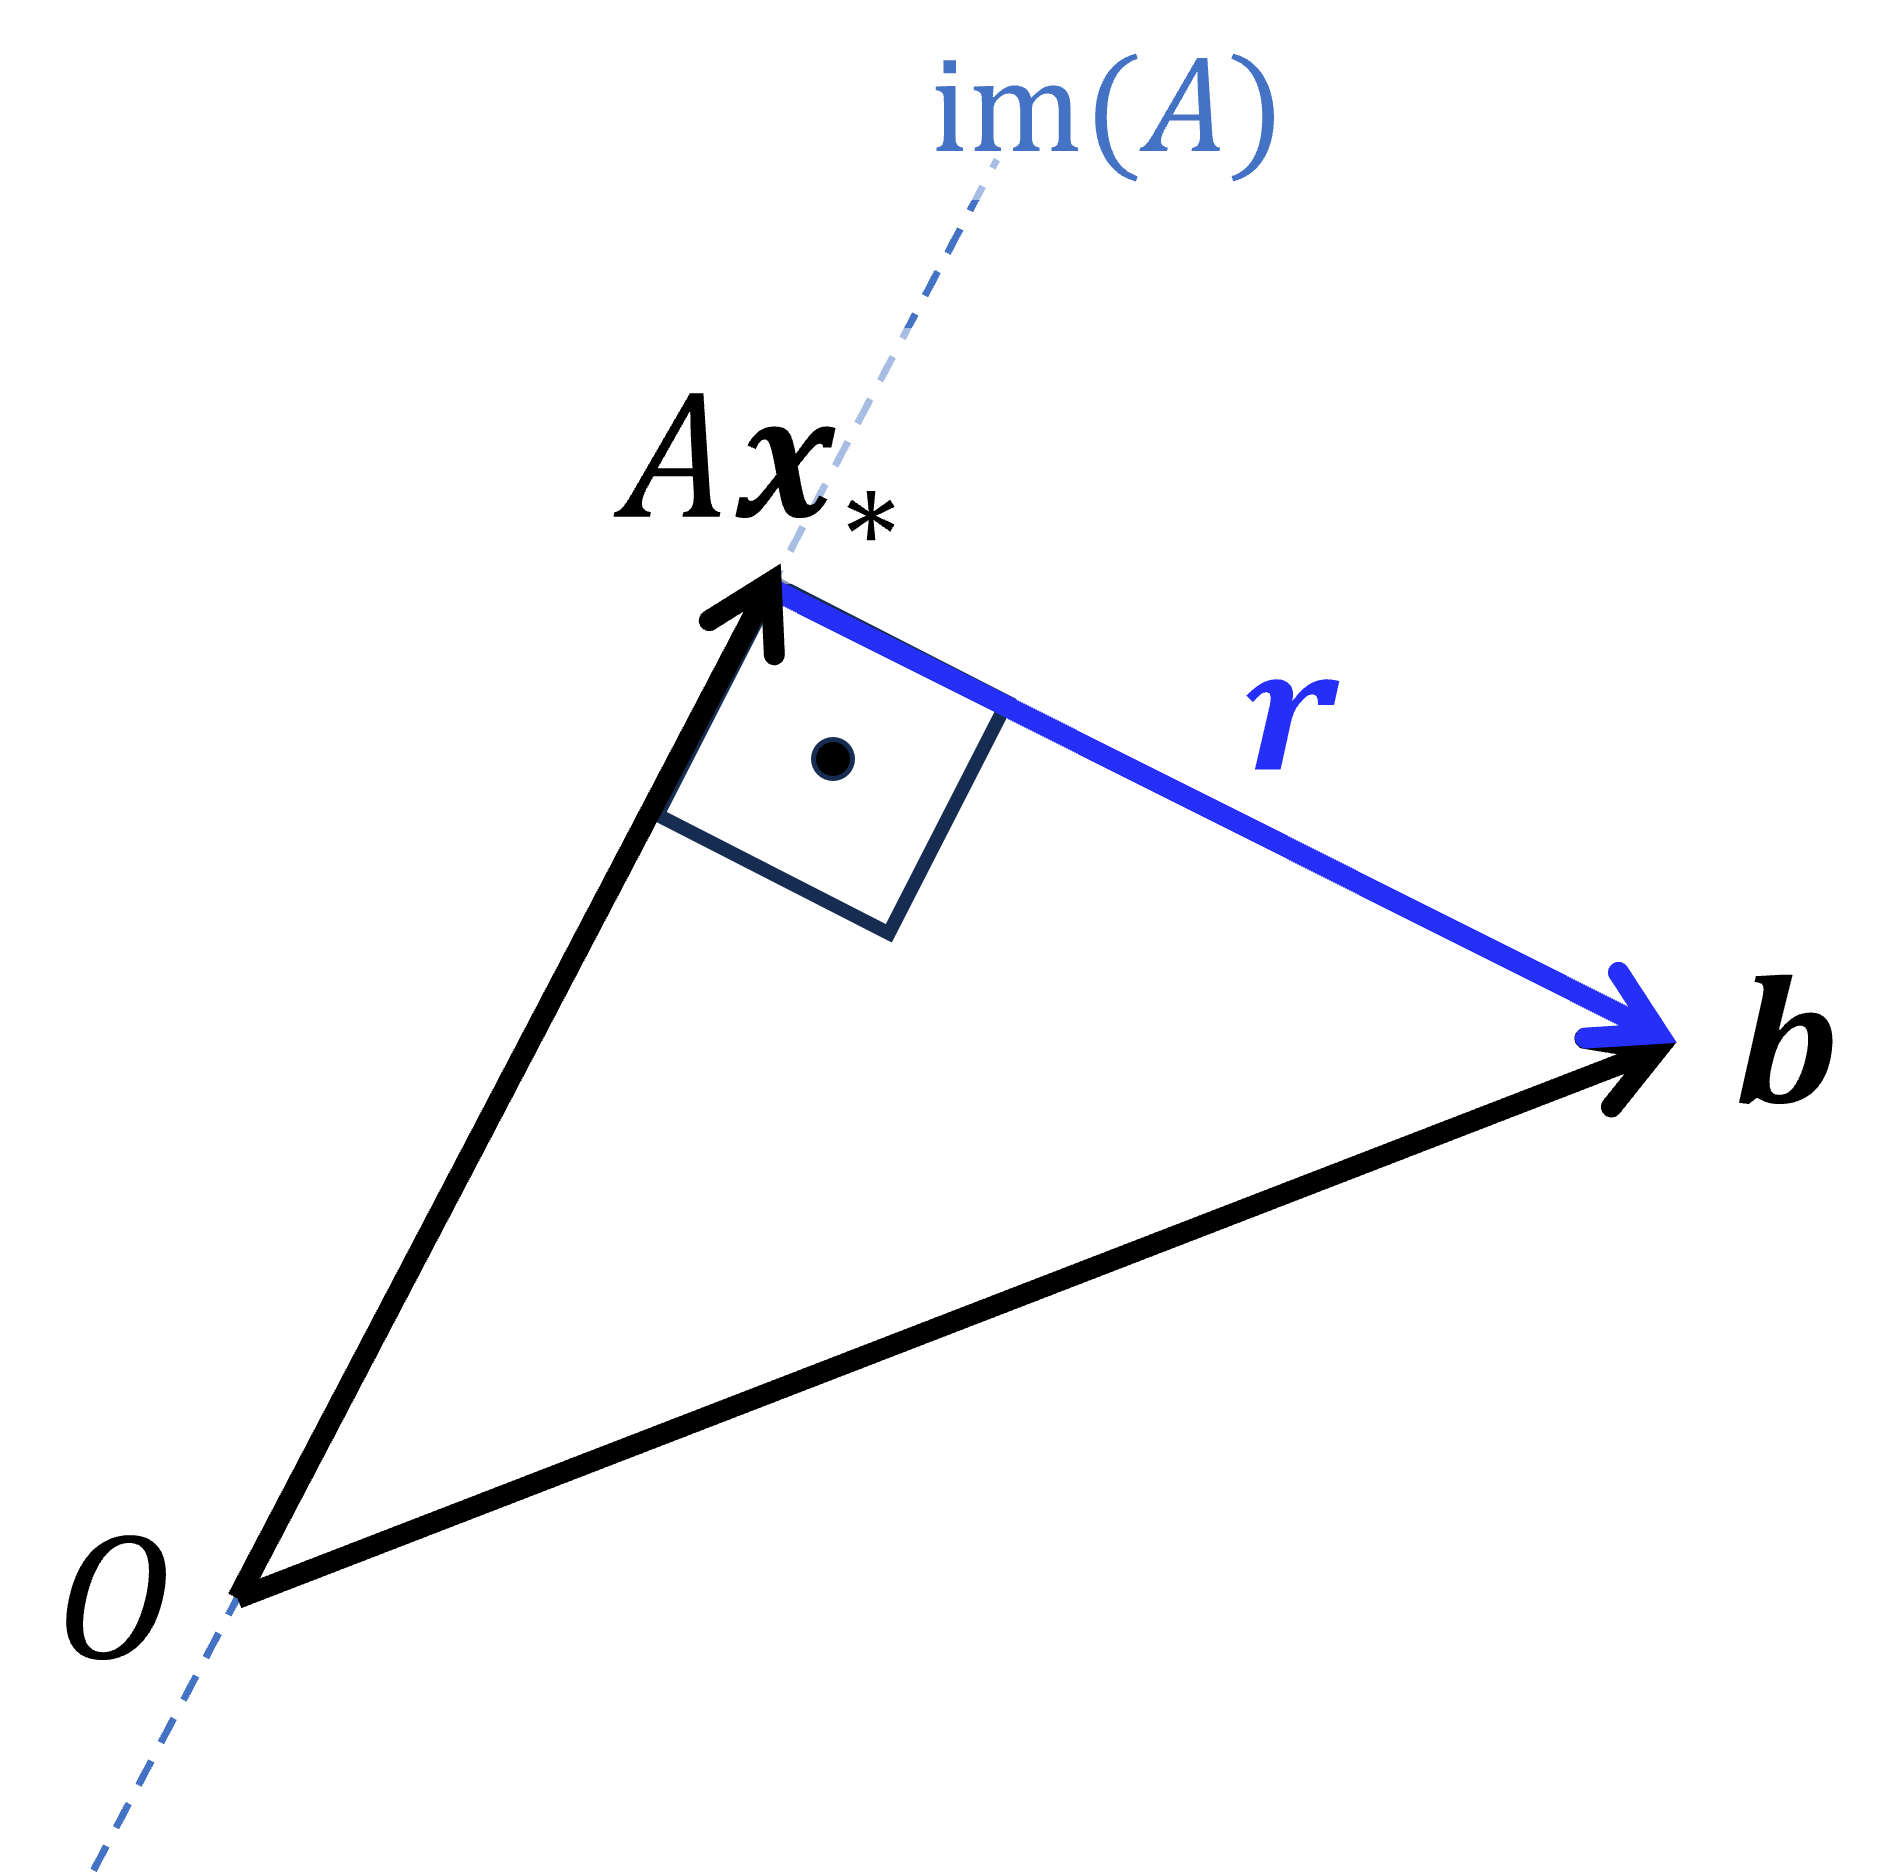
\includegraphics[width=\textwidth]{../Mathematik_2/Bilder/ausgleichsrechnung_residuum_orthogonal_zum_bildraum.png}
%\end{minipage}
%\begin{minipage}{0.65\textwidth}
%	Gegeben ist
%	\begin{itemize}
%		\item eine Matrix \(A\in\mathbb R^{n\times m}\) und
%		\item ein Vektor \(\boldsymbol b\in\mathbb R^n\) und
%		\item die L�sung \(\boldsymbol x_*\in\mathbb R^m\) der Normalengleichung.
%	\end{itemize}
%
%	Zeigen Sie, dass die folgenden Zusammenh�nge zwischen \(A\,\boldsymbol x_*\) und \(\boldsymbol r\) gelten:
%	\begin{itemize}
%		\item[(i)] Die L�nge des Residuums wird durch die L�sung der Normalengleichung minimiert:
%			\[ \| \boldsymbol r\| = \mathrm{min}  \; \Leftrightarrow \; A^\intercal \, A \, \boldsymbol x_* = A^\intercal \, \boldsymbol b \,.\]
%		\item[(ii)] Der Vektor \(A\,\boldsymbol x_*\) ist die Orthogonalprojektion von \(\boldsymbol b\) auf \(\mathrm{im}(A)\).
%	\end{itemize}
%\end{minipage}
%	\noindent \textbf{Hinweis:} Betrachten Sie die Funktion \(E: \boldsymbol x \mapsto \| A\,\boldsymbol x - \boldsymbol b\|^2\) und bestimmen Sie die station�ren Punkte.
%\end{exercisebox}
